% Options for packages loaded elsewhere
\PassOptionsToPackage{unicode}{hyperref}
\PassOptionsToPackage{hyphens}{url}
%
\documentclass[
  ignorenonframetext,
]{beamer}
\usepackage{pgfpages}
\setbeamertemplate{caption}[numbered]
\setbeamertemplate{caption label separator}{: }
\setbeamercolor{caption name}{fg=normal text.fg}
\beamertemplatenavigationsymbolsempty
% Prevent slide breaks in the middle of a paragraph
\widowpenalties 1 10000
\raggedbottom
\setbeamertemplate{part page}{
  \centering
  \begin{beamercolorbox}[sep=16pt,center]{part title}
    \usebeamerfont{part title}\insertpart\par
  \end{beamercolorbox}
}
\setbeamertemplate{section page}{
  \centering
  \begin{beamercolorbox}[sep=12pt,center]{part title}
    \usebeamerfont{section title}\insertsection\par
  \end{beamercolorbox}
}
\setbeamertemplate{subsection page}{
  \centering
  \begin{beamercolorbox}[sep=8pt,center]{part title}
    \usebeamerfont{subsection title}\insertsubsection\par
  \end{beamercolorbox}
}
\AtBeginPart{
  \frame{\partpage}
}
\AtBeginSection{
  \ifbibliography
  \else
    \frame{\sectionpage}
  \fi
}
\AtBeginSubsection{
  \frame{\subsectionpage}
}
\usepackage{lmodern}
\usepackage{amssymb,amsmath}
\usepackage{ifxetex,ifluatex}
\ifnum 0\ifxetex 1\fi\ifluatex 1\fi=0 % if pdftex
  \usepackage[T1]{fontenc}
  \usepackage[utf8]{inputenc}
  \usepackage{textcomp} % provide euro and other symbols
\else % if luatex or xetex
  \usepackage{unicode-math}
  \defaultfontfeatures{Scale=MatchLowercase}
  \defaultfontfeatures[\rmfamily]{Ligatures=TeX,Scale=1}
\fi
\usetheme[]{Madrid}
% Use upquote if available, for straight quotes in verbatim environments
\IfFileExists{upquote.sty}{\usepackage{upquote}}{}
\IfFileExists{microtype.sty}{% use microtype if available
  \usepackage[]{microtype}
  \UseMicrotypeSet[protrusion]{basicmath} % disable protrusion for tt fonts
}{}
\makeatletter
\@ifundefined{KOMAClassName}{% if non-KOMA class
  \IfFileExists{parskip.sty}{%
    \usepackage{parskip}
  }{% else
    \setlength{\parindent}{0pt}
    \setlength{\parskip}{6pt plus 2pt minus 1pt}}
}{% if KOMA class
  \KOMAoptions{parskip=half}}
\makeatother
\usepackage{xcolor}
\IfFileExists{xurl.sty}{\usepackage{xurl}}{} % add URL line breaks if available
\IfFileExists{bookmark.sty}{\usepackage{bookmark}}{\usepackage{hyperref}}
\hypersetup{
  pdftitle={Presentation},
  pdfauthor={Minsu Kim, Alona Muzikansky, Ariane Stark, Jadey Wu},
  hidelinks,
  pdfcreator={LaTeX via pandoc}}
\urlstyle{same} % disable monospaced font for URLs
\newif\ifbibliography
\usepackage{graphicx,grffile}
\makeatletter
\def\maxwidth{\ifdim\Gin@nat@width>\linewidth\linewidth\else\Gin@nat@width\fi}
\def\maxheight{\ifdim\Gin@nat@height>\textheight\textheight\else\Gin@nat@height\fi}
\makeatother
% Scale images if necessary, so that they will not overflow the page
% margins by default, and it is still possible to overwrite the defaults
% using explicit options in \includegraphics[width, height, ...]{}
\setkeys{Gin}{width=\maxwidth,height=\maxheight,keepaspectratio}
% Set default figure placement to htbp
\makeatletter
\def\fps@figure{htbp}
\makeatother
\setlength{\emergencystretch}{3em} % prevent overfull lines
\providecommand{\tightlist}{%
  \setlength{\itemsep}{0pt}\setlength{\parskip}{0pt}}
\setcounter{secnumdepth}{-\maxdimen} % remove section numbering

\title{Presentation}
\author{Minsu Kim, Alona Muzikansky, Ariane Stark, Jadey Wu}
\date{}

\begin{document}
\frame{\titlepage}

\begin{frame}{Alona: Examining the relationship between Duration of
Arterial Hypertension and CHF}
\protect\hypertarget{alona-examining-the-relationship-between-duration-of-arterial-hypertension-and-chf}{}

\begin{center}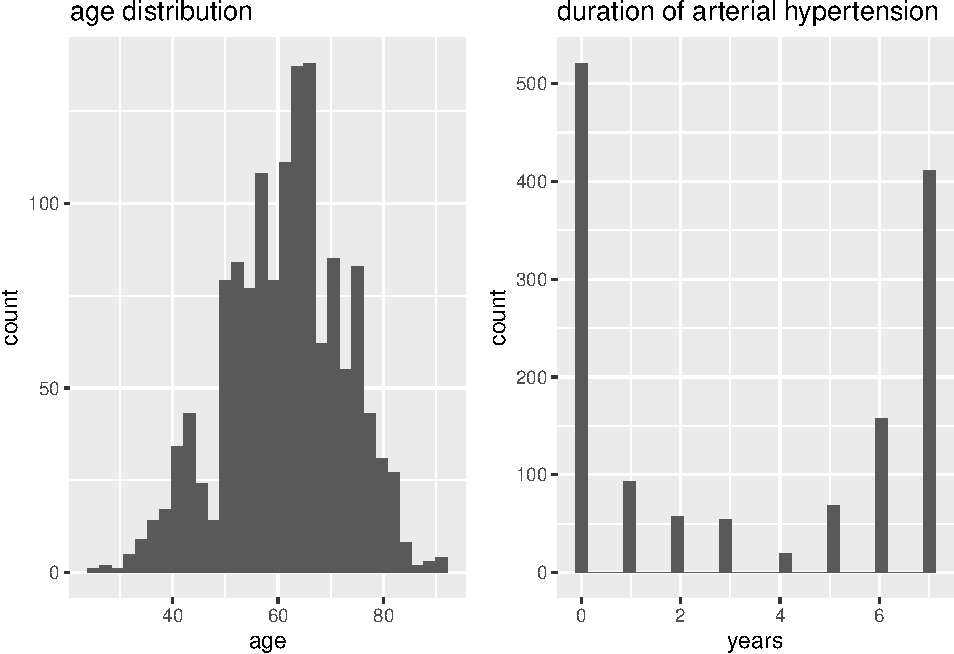
\includegraphics{Presentation-a_files/figure-beamer/unnamed-chunk-2-1} \end{center}

\end{frame}

\begin{frame}{}
\protect\hypertarget{section}{}

\begin{itemize}
\item
  The two classes of CHF have similar count distributions across the
  levels of duration of arterial hypertension.
\item
  We will further test the hypothesis that there is an association
  between the two variables
\end{itemize}

\end{frame}

\begin{frame}{Inference for contigency table.}
\protect\hypertarget{inference-for-contigency-table.}{}

\begin{table}

\caption{\label{tab:unnamed-chunk-3}Duration of Arterial Hypertension by Chronic Heart Failure}
\centering
\begin{tabular}[t]{l|r|r}
\hline
  & No & Yes\\
\hline
None & 401 & 120\\
\hline
1 & 72 & 21\\
\hline
2 & 47 & 10\\
\hline
3 & 42 & 12\\
\hline
4 & 15 & 4\\
\hline
5 & 48 & 20\\
\hline
6-10 & 120 & 37\\
\hline
>=10 & 307 & 104\\
\hline
\end{tabular}
\end{table}

\end{frame}

\begin{frame}{Examining the Standerdized residuals.}
\protect\hypertarget{examining-the-standerdized-residuals.}{}

\includegraphics{Presentation-a_files/figure-beamer/unnamed-chunk-4-1.pdf}

\end{frame}

\begin{frame}[fragile]{}
\protect\hypertarget{section-1}{}

For Ix2 tables, testing for a linear trend in either response category,
we use the Cochran-Armitage trend test.

\begin{verbatim}
## 
##  Cochran-Armitage test for trend
## 
## data:  dlitag
## Z = -0.99455, dim = 8, p-value = 0.32
## alternative hypothesis: two.sided
\end{verbatim}

Issues to consider: Ordinal variable with unequal intervals so trend
test on the original classification provides information about the
direction but ignores the unequal spacing in the last two categories.

\end{frame}

\begin{frame}{Logistic Regression model}
\protect\hypertarget{logistic-regression-model}{}

\begin{table}

\caption{\label{tab:unnamed-chunk-6}Parameter Estimates for Logit link}
\centering
\begin{tabular}[t]{l|r|r|r|r}
\hline
  & Estimate & Std. Error & z value & Pr(>|z|)\\
\hline
(Intercept) & -1.2283412 & 0.0915051 & -13.4237468 & 0.0000000\\
\hline
`Duration of Arterial hypertension` & 0.0138949 & 0.0143812 & 0.9661872 & 0.3339505\\
\hline
\end{tabular}
\end{table}

\end{frame}

\begin{frame}{Goodness of fit tests for the fitted models}
\protect\hypertarget{goodness-of-fit-tests-for-the-fitted-models}{}

For the logit model:

\begin{itemize}
\tightlist
\item
  \(G^2\) = 2.4236058
\item
  df = 6
\item
  p-value = 0.8769175
\end{itemize}

For the linear model:

\begin{itemize}
\tightlist
\item
  \(G^2\) = 2.4236058
\item
  df = 6
\item
  p-value = 0.8769175
\end{itemize}

\end{frame}

\begin{frame}{}
\protect\hypertarget{section-2}{}

Predicted probabilities for the fitted models and the observed data.

\end{frame}

\begin{frame}{Sub-analsis}
\protect\hypertarget{sub-analsis}{}

We tested the Linear model for the subset: Duration of arterial
hypertension \(\in[1 - 5]\)

\begin{table}

\caption{\label{tab:unnamed-chunk-10}Parameter Estiamtes for subset analysis}
\centering
\begin{tabular}[t]{l|r|r|r|r}
\hline
  & Estimate & Std. Error & z value & Pr(>|z|)\\
\hline
(Intercept) & 0.1850895 & 0.0483670 & 3.826774 & 0.0001298\\
\hline
DLIT\_AG\_N & 0.0167632 & 0.0161478 & 1.038107 & 0.2992204\\
\hline
\end{tabular}
\end{table}

\end{frame}

\begin{frame}{}
\protect\hypertarget{section-3}{}

Predicted probabilities
\includegraphics{Presentation-a_files/figure-beamer/unnamed-chunk-11-1.pdf}
The p-value for the goodness of fit went down sharply (0.16) but still
didn't reach significance level to reject the null of no-fit.

\end{frame}

\begin{frame}{Conclusions}
\protect\hypertarget{conclusions}{}

\begin{itemize}
\tightlist
\item
  There is no significant association between CHF and the duration of
  arterial hypertension.
\item
  By itself, duration of arterial hypertension is not predictive of CHF.
\end{itemize}

\end{frame}

\end{document}
